\documentclass{article}

\usepackage{amsfonts}
\usepackage{amsmath}
\usepackage{interval}
\usepackage[T1]{fontenc}
\usepackage{pdftexcmds}
\usepackage{pgfplots}
\pgfplotsset{compat=1.8}

\begin{document}

\title{A Model of Double-Entry Bookkeeping Systems}
\author{}
\date{}
\maketitle

\section{Double-Entry Bookkeeping Space}

A double-entry bookkeeping information system can be viewed as a three dimensional space,
where each dimension represents:

\begin{itemize}
	\item $a \in A$, where $A$ is a subset of a predefined set of accounts.
	\item $d \in D$, where $D$ is a subset of all possible dates
		in the Gregorian calendar.
	\item $m \in M$, where $M$ is a subset of all possible discrete points in time, given a precision.
\end{itemize}

Figure~\ref{fig:deb-space-sample} shows a \emph{double-entry bookkeeping space} sample, 
where each cube represents a integer value different from zero.
Consider the cubes $(4,1,1)$ and $(6,1,1)$. They share the same moment 
and date---the only difference are the accounts. 
We can interpret this pair of cubes as a transaction recorded in the system,
with one cube representing the debit and another representing the credit.

\begin{figure}[h]
\centering
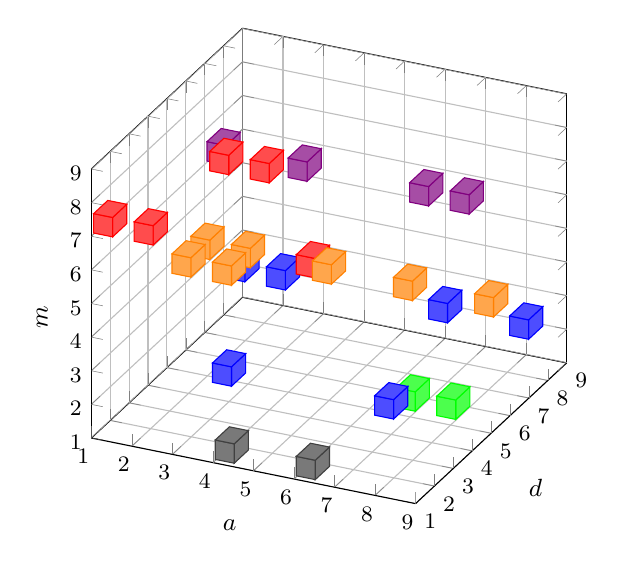
\begin{tikzpicture}
\begin{axis}[
	% view={120}{40},
	small,
	height=3in,
	width=3in,
	grid=major,
	xlabel=$a$,
	ylabel=$d$,
	zlabel=$m$,
	xmin=1,xmax=9,
    ymin=1,ymax=9,
    zmin=1,zmax=9,
    xtick={1,2,...,10},
    ytick={1,2,...,10},
    ztick={1,2,...,10},
	colormap={summap}{
        color=(darkgray); color=(blue);
        color=(green); color=(yellow)
        color=(orange) color=(violet)
        color=(red)
    },
    scatter/use mapped color={
        draw=mapped color,fill=mapped color!70},
]
\addplot3[only marks,scatter,mark=cube*,mark size=7] coordinates {
            (1,9,2) (2,9,2) (6,9,2) (8,9,2)
            (7,8,6) (1,8,6) (2,6,7) (3,6,7)
            (1,2,7) (2,2,7) (6,2,7) (2,5,5)
            (3,5,5) (5,5,5) (7,5,5) (9,5,5)
            (3,8,6) (6,8,6) (2,4,5) (3,4,5)
            (8,3,3) (9,3,3) (3,4,2) (7,4,2)
            (4,2,1) (6,2,1)
        };
\end{axis}
\end{tikzpicture}
\label{fig:deb-space-sample}
\caption{A \emph{double-entry bookkeeping space} sample.}
\end{figure}

As, by definition, a double-entry transaction must have debits' sum
equals to credits' sum, we can deduce that the values for both
cubes are the same, in this example.

More specifically, we can have a \emph{double-entry bookkeeping space} 
represented by a three dimensional array $S$:
\begin{equation}
	\label{eq:space}
	S = \left(s_{ijk}\right), 
	\; 1 \leq i \leq |A|, \; 1 \leq j \leq |D|, \; 1 \leq k \leq |M|, 
	\; s_{ijk} \in \mathbb{Z}
\end{equation}

Satisfying the following property:

\begin{equation}
	\label{eq:property}
	\forall j \; \forall k, \sum_{i=1}^{|A|}{s_{ijk}} = 0
\end{equation}

The equations~\eqref{eq:space}~and~\eqref{eq:property}
assume that debits are represented by positive integers
and credits by negative integers.

\section{Operations}

A \emph{double-entry bookkeeping space} supports the following operations:

\begin{description}
	\item[\textsc{Insert}$(S,T)$] inserts the two dimensional array 
	$T=\left(t_{ij}\right)$ into the space,
		such that the set $M$ of the space $S$ will be replaced by $M'$, 
		where $|M'| = |M|+1$, and:
		\[
			s_{ijk} = t_{ij}, \; k = |M'|
		\]

	\item[\textsc{Projection}$(S, \langle b_1, e_1 \rangle, \; \cdots,
		\langle b_n, e_n \rangle)$] 
		returns a two dimensional array $P=\left(p_{qr}\right)$ such that:
		\[
			p_{qr} = \sum_{j=b_r}^{e_r}{\sum_{k=1}^{|M|}{S_{qjk}}}, 
				\; 1 \leq q \leq |A|, \; 1 \leq r \leq n
		\]

	\item[\textsc{Slice}$(S, A', \langle d_b,d_e \rangle, \langle m_b,m_e \rangle)$] 
		returns a potentially smaller space $S'=\left(s'_{pqr}\right)$, such that:
		\[
			\begin{array}{l}
				s'_{pqr} = s_{ijk}, \\
				1 \leq p \leq |A'|, \;1 \leq q \leq d_e-d_b+1, \; 1 \leq r \leq m_e-m_b+1, \\
				A'_p = A_i, \; d_b \leq j \leq d_e, \; m_b \leq k \leq m_e
			\end{array}			
		\]

\end{description}

\end{document}